\documentclass[tikz]{standalone}
\usepackage{fontspec}
\renewcommand*{\familydefault}{\sfdefault}
\usepackage{standalone}
\usepackage{amssymb}
\usetikzlibrary{decorations}
\usetikzlibrary{arrows.meta, decorations.pathmorphing, decorations.pathreplacing, shapes.geometric}
\usetikzlibrary{mindmap}

\begin{document}

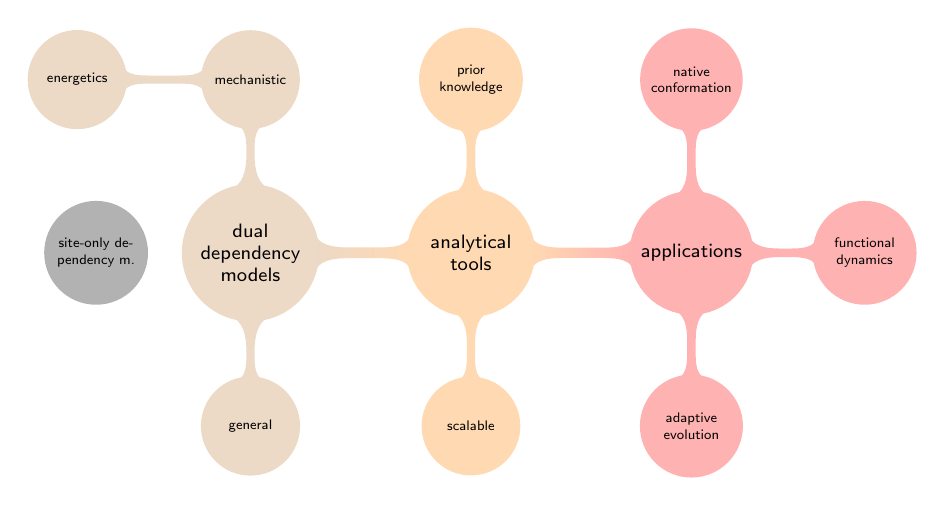
\begin{tikzpicture}[small mindmap, concept color=brown!30!white, text=black]

\node[concept, level 1 concept] (new-mod) {dual dependency models}
[clockwise from=45]
child[level 2 concept, grow=-90] {node[concept] {general}
}
child[level 2 concept, grow=+90] {node[concept] {mechanistic}
    child[grow=180] {node[concept] {energetics}}
}
child[grow=0, concept color=orange!30!white] {node[concept] {analytical tools}
    child[level 2 concept, grow=+90] {node[concept] {prior knowledge}}
    child[level 2 concept, grow=-90] {node[concept] {scalable}}
child[level 1 concept, grow=0, concept color=red!30!white] {node[concept] {applications}
    child[level 2 concept, grow=+90] {node[concept] {native conformation}}
    child[level 2 concept, grow=+0] {node[concept] {functional dynamics}}
    child[level 2 concept, grow=-90] {node[concept] {adaptive evolution}}
}
}
;
\node[extra concept, concept color=black!30!white, left=0.5 cm] at
(new-mod.west) {site-only dependency m.};

\end{tikzpicture}

\end{document}
